\section{Introdução} 
\subsection{Definição justificada dos objetivos e da sua relevância}
A palavra ``computador'' é usada desde o século XVII, tendo a sua primeira referência escrita datada de 1613. No entanto, por muito tempo ``computador'' não tinha o mesmo significado que leva hoje, sendo utilizado, até a década de 1940, para se referir à profissão de alguém que calcula, segundo o dicionário Michaelis: ``Aquele ou aquilo que calcula baseado em valores digitais; calculador, calculista'' \cite{4}.

Tendo em vista o antigo significado atribuído à palavra ``computador'', pode-se questionar sobre como passamos a utilizar uma palavra antes atribuída à pessoas, para se referir à máquinas. Pode-se sugerir que a transição de significado acompanhou o estudo de Alan Turing (Reino Unido, 1912-1954) – um matemático, lógico, criptógrafo e herói de guerra – que tinha como objetivo compreender aquilo que podia ou não ser calculado, resultando no desenvolvimento da Maquina de Turing – também conhecida como ``Maquina Universal'' – , que veio a ser considerada o modelo mais poderoso de computador. O desenvolvimento de seu trabalho publicado em 1937, trouxe muitas contribuições para o desenvolvimento da computação, sendo o estudo que originou os computadores e celulares que você, leitor, pode estar usando para ler o presente trabalho. Assim, entende-se a importância de iniciar este estudo a partir de suas contribuições para a computação, compreendendo a constituição e funcionamento da máquina que serviu como base para os demais avanços computacionais. 

O modelo matemático da Máquina de Turing foi desenvolvido a partir de três principais componentes: fita infinita; cabeçote; e a máquina de estado finito; – sendo similar a um autômato finito\footnote{Um sub-tópico da Ciência da computação teórica, também chamado máquina de estados finita determinística — é uma máquina de estados finita que aceita ou rejeita cadeias de símbolos gerando um único ramo de computação para cada cadeia de entrada.}, porém com uma memória ilimitada e irrestrita, ilustrada na figura \ref{turing_machine} abaixo.

\vspace{1cm}
\begin{figure}[H] \centering 
  \makebox[\textwidth][c]{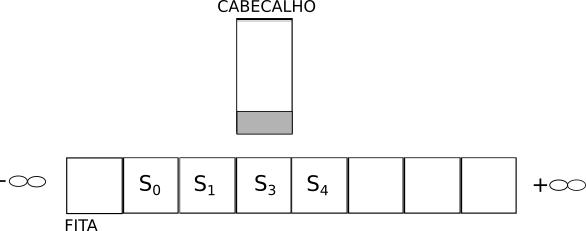
\includegraphics[width=0.8\textwidth]{turing_machine.png}}
  \caption{\label{turing_machine} Desenho esquemático Máquina de Turing} 
\end{figure}

Neste modelo, a fita infinita é dividida em células, cada uma contendo um símbolo de um alfabeto finito. O cabeçote é responsável por se deslocar para a direita ou para a esquerda e efetuar a leitura ou escrita em uma célula. Este processo é ilustrado pelo Prof. Dr. Fabio Gagliardi Cozman \cite{7} da seguinte forma:

\begin{enumerate}
  \item Inicialmente a fita contém somente a cadeia de entrada (dados originários do programa), disposta no ``meio''\footnote{Meio é algo abstrato nesse sentido, pois não existe meio de um valor infinito} da fita, com o cabeçote posicionado no início da cadeia, tendo o resto das células da fita vazias;
  \item Para armazenar algo, a máquina escreve na fita;
  \item O cabeçote pode ser movido livremente para a esquerda ou direita, afim de ler ou escrever valores em qualquer célula;
  \item As saídas ``aceita'' e ``rejeita'' são obtidas ao entrar nos estados de aceitação e rejeição;
  \item Se não entrar em um estado de aceitação ou rejeição, continuará sua computação para sempre, em ``loop infinito''.
\end{enumerate}

Assim, a partir desse funcionamento, o modelo computacional de Turing possibilitou três operações fundamentais básicas: a leitura, a escrita e a movimentação.   

Após aproximadamente uma década, em 1946, o primeiro computador digital eletrônico de grande escala foi criado pelos cientistas norte-americanos, John Presper Eckert e John W. Mauchly, da Electronic Control Company. Sendo a primeira implementação digital-eletrônica da máquina de Turing, o ENIAC (Electrical Numerical Integrator and Calculator) foi mais um marco da evolução da tecnologia. Ao final dos seus 10 anos de operação, em 1956, o ENIAC continha 20.000 tubos de vácuo, 7.200 diodos de cristal, 1.500 relés, 70.000 resistores, 10.000 capacitores e aproximadamente 5.000.000 juntas soldadas à mão. Ele pesava mais de 27 toneladas, tinha aproximadamente 2,4m × 0,9m × 30m de tamanho, consumia 150 kW de eletricidade e ocupava 167 m² \cite{2}, tendo a sua disposição ilustrada na figura \ref{ENIAC_floor_layout} abaixo. 

\vspace{1cm}
\begin{figure}[H] \centering 
 \makebox[\textwidth][c]{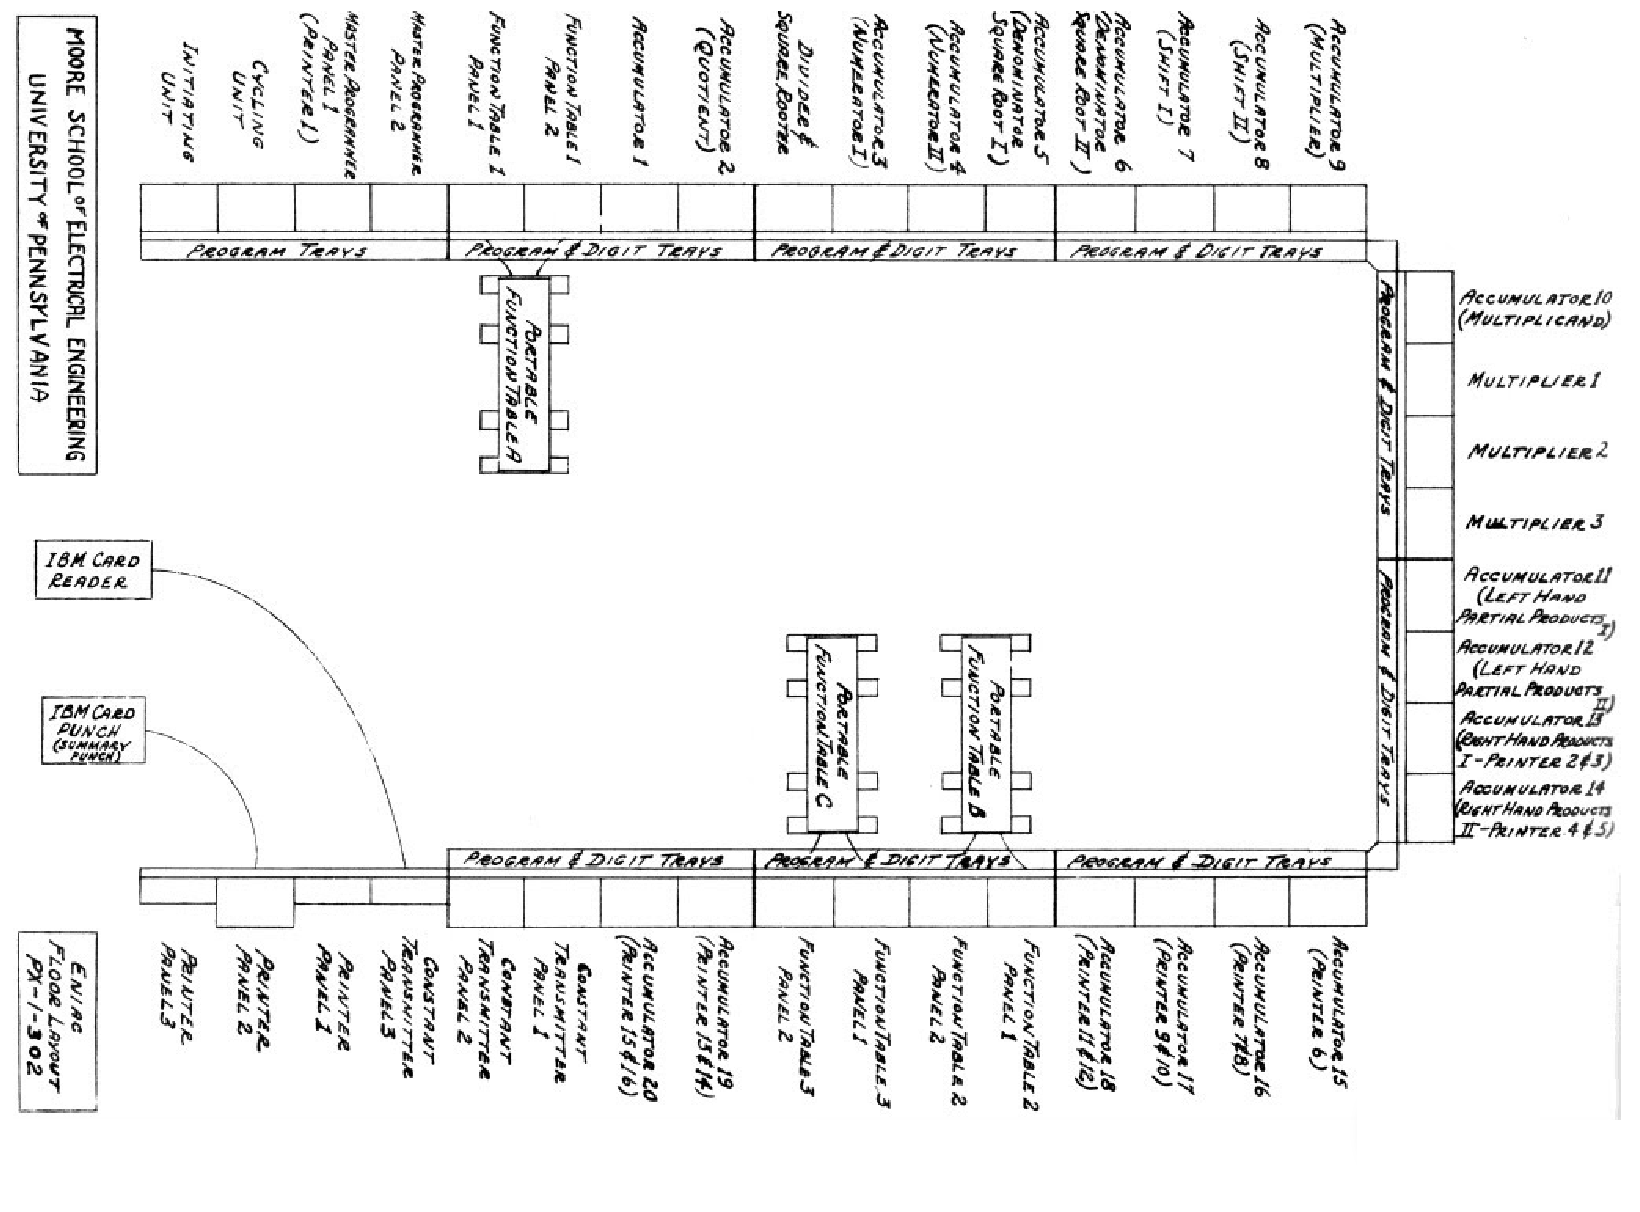
\includegraphics[width=0.8\textwidth]{ENIAC_floor_layout.png}}
  \caption{\label{ENIAC_floor_layout} Desenho esquemático do ENIAC/US Center for Military History — Adele Goldstine} 
\end{figure}

A partir do ENIAC, as possibilidades tecnológicas tomaram uma nova proporção. Em 1969, apenas 13 anos após o desligamento do primeiro computador digital eletrônico, o computador de bordo da Apollo 11 — missão que levou o homem à Lua — tinha 32.768 bits\footnote{Para uma explicação elaborada sobre bits refira-se ao capítulo \ref{classic_comp} pagina \pageref{bits}} de RAM, o suficiente para armazenar apenas um texto não formatado, com cerca de 2.000 palavras. O que contrasta com o Iphone XS com 4gb de RAM, que em 2018, tinha cerca de 1 milhão de vezes mais de memória que o Apollo Guinche Computer \cite{5}.

Durante o século XX, além do aumento do poder computacional dos dispositivos, outro fator impactante foi a refatoração de seus tamanhos. Assim, com tecnologias wearables\footnote{A tecnologia em questão não somente pode ser usada como uma peça de roupa ou um acessório, como também tem que possuir características que a conectem a outros aparelhos ou à internet.}, os computadores se tornam ativamente presentes no cotidiano. 

Levando em consideração o rápido avanço e desenvolvimento computacional, entende-se que os computadores trazem benefícios à sociedade, seja facilitando a comunicação e o compartilhamento de conhecimentos, como em outros aspectos. No entanto, a agilidade dessas \textbf{transformações da tecnologia da computação}, gera grandes expectativas e incertezas sobre o que ainda está por vir, tanto nas questões de mudanças tecnológicas quanto nos impactos na sociedade.

Tendo em vista a incerteza que acompanha o futuro da computação e de seus próximos avanços, a presente pesquisa se propõe a estudar os conceitos da física clássica e da física quântica aplicados à computação, além do estudo dos princípios da criptografia\footnote{Criptografia é um sistema de algoritmos matemáticos que codificam dados para que só o destinatário possa ler.}. Com base nesses conceitos será prototipado um computador clássico de 8 bits em hardware usando apenas portas lógicas simples, de forma a possibilitar uma ilustração clara do funcionamento. Junto a isso será desenvolvida uma aplicação web que ilustra o funcionamento de um processador quântico. Ao final, conceitos de criptografia serão utilizados para exemplificar possíveis mudanças sociais que os próximos avanços tecnológicos podem gerar.

\subsection{Metodologia a ser empregada}
Tem-se que para a realização da presente pesquisa de iniciação científica, é indispensável a realização de uma revisão bibliográfica, afim de recuperar e se aprofundar no conhecimento cientifico já produzido. Segundo Telma Cristiane Sasso de Lima, o conhecimento da realidade não é apenas a simples transposição dessa realidade para o pensamento, mas sim a reflexão crítica, que se dá a partir de um conhecimento acumulado que irá gerar uma síntese, o concreto pensado \cite{1}. E também a utilização do processo científico para a elaboração e efetivação do projeto em si. Ambas metodologias citadas acima são cruciais para o desenvolvimento do relatório final na área de pesquisa em computação, já que em grande parte dos estudos, a utilização do processo científico é frequentemente utilizada para um maior entendimento da obra e a construção do projeto se tornar mais facilmente executável.

Assim, para o desenvolvimento da entrega do protótipo — computador de 8-bits — e para o simulador do computador quântico web, a principal metodologia utilizada será Project Based Learnig (PBL). De acordo com David Van Andel, o PBL envolve os alunos em um processo rigoroso de investigação, onde eles fazem perguntas, encontram recursos e aplicam informações para resolver problemas do mundo real \cite{3}. Assim, entende-se que esta é a melhor metodologia para desenvolver um protótipo físico de um computador e programar um site.

Nos dois capítulos a seguir, \ref{classic_comp} e \ref{quantum_comp}, respectivamente Computação clássica e Computação quântica é apresentada a revisão bibliográfica 

% \subsection{Considerações finais do capítulo}

\newpage

